% universal settings
\documentclass[a5paper,11pt,twoside,onecolumn,openany,extrafontsizes,final]{memoir}%,showtrims pour les traits de coupe
\epigraphfontsize{\small\itshape}
\setlength\epigraphwidth{8cm}
\setlength\epigraphrule{0pt}
%=======================
%Pour le fond perdu  prépress
%\setstocksize{224.8mm}{162.9mm}
%\settrimmedsize{210mm}{148mm}{*}
%\settrims{7.4mm}{7.45mm}
\quarkmarks
%=====================
\usepackage[utf8]{inputenc}
\usepackage[T1]{fontenc}
\usepackage[ngerman]{babel}
\usepackage[osf]{Alegreya,AlegreyaSans}
\usepackage{graphicx}
\usepackage[labelformat=empty,textfont={it}]{caption}
\usepackage{pdfpages}
\usepackage[
    type={CC},
    modifier={by-nc-nd},
    version={4.0},
]{doclicense}

% PACKAGE DEFINITION
% typographical packages
\usepackage{microtype} % for micro-typographical adjustments
\usepackage{setspace} % for line spacing
\usepackage{lettrine} % for drop caps and awesome chapter beginnings
\usepackage{titlesec} % for manipulation of chapter titles
\usepackage{enumitem}
% for placeholder text
\usepackage{lipsum} % to generate Lorem Ipsum

% other
\usepackage{calc}
\usepackage{hologo}
\usepackage[hidelinks]{hyperref}
\urlstyle{tt}
%\usepackage{showframe}

%footnote numbering
\usepackage{chngcntr}
\counterwithout*{footnote}{chapter}

% PHYSICAL DOCUMENT SETUP
% media settings
%\setstocksize{210mm}{148mm}
%\settrimmedsize{210mm}{148mm}{*}
%\setbinding{8mm}
%\setlrmarginsandblock{15mm}{2.1cm}{*}
%\setulmarginsandblock{15mm}{2.1cm}{*}
\semiisopage[12]
% custom second title page
\makeatletter
\newcommand*\halftitlepage{\begingroup % Misericords, T&H p 153
  \setlength\drop{0.1\textheight}
  \begin{center}
  \vspace*{\drop}
  \rule{\textwidth}{0in}\par
  {\Large\textsc\thetitle\par}
  \rule{\textwidth}{0in}\par
  \vfill
  \end{center}
\endgroup}
\makeatother

% custom title page
\thispagestyle{empty}
\makeatletter
\newlength\drop
\newcommand*\titleM{\begingroup % Misericords, T&H p 153
  \setlength\drop{0.15\textheight}
  \begin{center}
  \vspace*{\drop}
  \rule{\textwidth}{0in}\par
  {\HUGE\textsc\thetitle\par}
  \rule{\textwidth}{0in}\par
  {\Large\textit\theauthor\par}
  \vfill
  {\Large\scshape\press}
  \end{center}
\endgroup}
\makeatother

% chapter title manipulation
% padding with zero
%\renewcommand*\thechapter{\ifnum\value{chapter}<10 0\fi\arabic{chapter}}
% chapter title display
\titleformat
{\chapter}
[display]
{\normalfont\scshape\huge}
{\HUGE\thechapter\centering}
{0pt}
{\vspace{5pt}\centering}[\vspace{25pt}]

% typographical settings for the body text
\setlength{\parskip}{0em}
\linespread{1.09}

% HEADER AND FOOTER MANIPULATION
  % for normal pages
  \nouppercaseheads
  \headsep = 0.22in
  \makepagestyle{mystyle} 
  \setlength{\headwidth}{\dimexpr\textwidth+\marginparsep+\marginparwidth\relax}
  \makerunningwidth{mystyle}{\headwidth}
  \makeevenhead{mystyle}{}{\textsf{\scriptsize\scshape\thetitle}}{}
  \makeoddhead{mystyle}{}{\textsf{\scriptsize\scshape\leftmark}}{}
  \makeevenfoot{mystyle}{}{\textsf{\scriptsize\thepage}}{}
  \makeoddfoot{mystyle}{}{\textsf{\scriptsize\thepage}}{}
  \makeatletter
  \makepsmarks{mystyle}{%
  \createmark{chapter}{left}{nonumber}{}{}}
  \makeatother
  % for pages where chapters begin
  \makepagestyle{plain}
  \makerunningwidth{plain}{\headwidth}
  \makeevenfoot{plain}{}{}{}
  \makeoddfoot{plain}{}{}{}
  \pagestyle{mystyle}
% END HEADER AND FOOTER MANIPULATION

% table of contents customisation
\renewcommand\contentsname{\normalfont\scshape Contents}
\renewcommand\cftchapterfont{\normalfont}
\renewcommand{\cftchapterpagefont}{\normalfont}
\renewcommand{\printtoctitle}{\centering\Huge}



% layout check and fix
\checkandfixthelayout
\fixpdflayout

%\setsecnumdepth{none}
%\maxsecnumdepth{none}

% defining the title and the author

\title{Inge}
\author{\Huge Ingeborg Sader}
\newcommand{\press}{Kurzgeschichten}

\setlength\parindent{0pt}

% BEGIN THE DOCUMENT
\begin{document}
\pagestyle{empty}
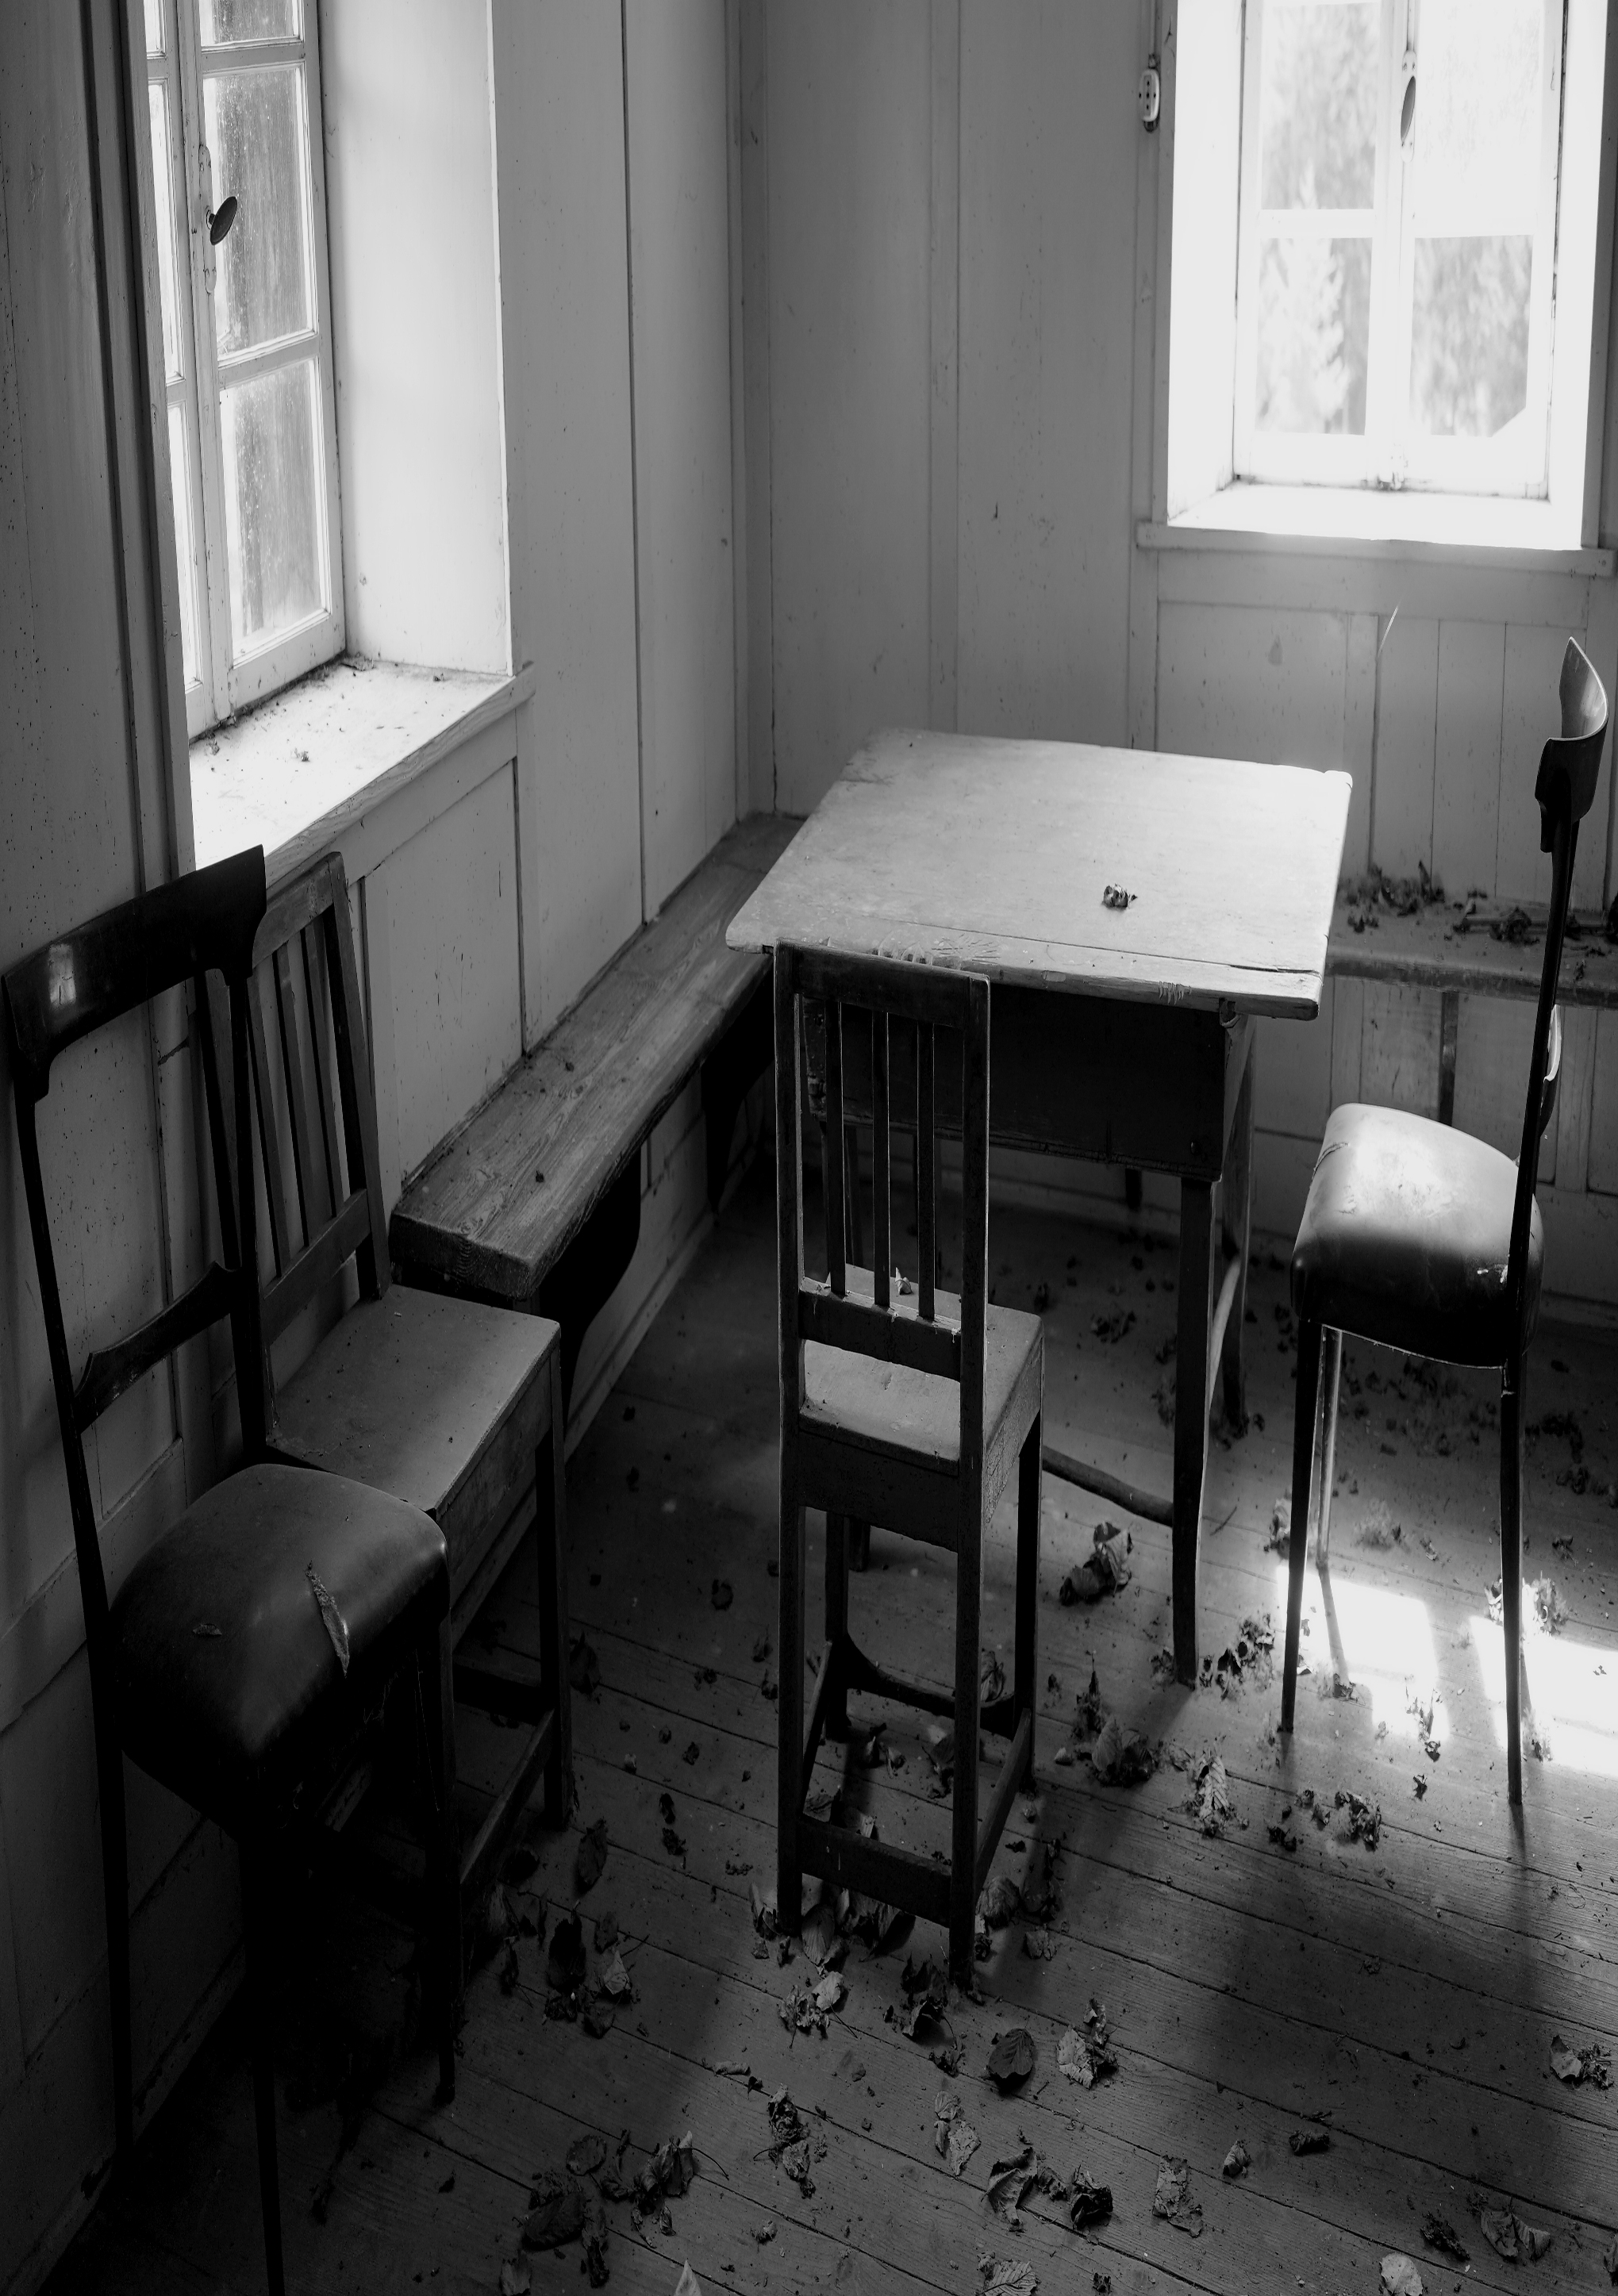
\includepdf{Illustrations/titel.jpg}
%\includepdf{Illustrations/carte_zad.jpg}
% the half title page
%\halftitlepage
%\cleardoublepage
% the title page
\titleM
\vspace{2\baselineskip}
%\par
\vspace{\baselineskip}
\begin{center}
\begin {tabular}{lr}
Erste Auflabge: & 24. Dezember 2020\\
%Deuxième impression avec corrections: & 10 novembre 2017 \\
%Deuxième édition: & 24 novembre 2017\\
\end{tabular}
\end{center}
\vspace{2\baselineskip}
\doclicenseThis
\vspace*{\baselineskip}
%\centerline{\textit{Retrouvez ce livre au format numérique au} \url{nathanaelnoi@gmail.com}} 
%%\centerline{\url{http://livretzad.lamad.net}}
\clearpage

% begin front matter
\frontmatter
\pagestyle{mystyle}
% preface
\chapter{Vorwort}

Viktoria schreibt Vorwort

%\newpage\phantom{blabla}

 \thispagestyle{empty}
    \null\vspace{\stretch {1}}
        \begin{flushright}
                Ich widme di.
        \end{flushright}
\vspace{\stretch{2}}\null
  \include{Inge/content/frontmatter/abstract}
    \newenvironment{acknowledgements}%
    {\cleardoublepage\thispagestyle{empty}\null\vfill\begin{center}%
    \bfseries Danksagung\end{center}}%
    {\vfill\null}
        \begin{acknowledgements}
        Wem möchtest du danken?............................................
        \end{acknowledgements}
    \include{Inge/content/frontmatter/preface}
\clearpage
\tableofcontents*


% begin main matter
\mainmatter
\sloppybottom
\chapter{„Vergelts Gott“}
%\vspace{\baselineskip}
\chapterprecishere{``
Wenn dich die Welt aus ihren Toren stößt, 
So gehe ruhig fort, und laß das Klagen.
 Sie hat durch die Verstoßung dich erlöst
 und ihre Schuld an dir nun selbst zu tragen."\par\raggedleft--- \textup{Karl May, Im Reiche des silbernen Löwen}}
\lettrine{D}{er} kleine Hans durchstrich wie ein verletztes Tier das Gehölz. Mit vorsichtigen Schritten befühlten seine nackten Füße einmal das weichfeuchte Moos, dann die Nadelflecken unterhalb der Waldungen des auffallenden Losers nördlich des großen Sees in Altaussee. Hier ging er selbst für sich. Der Wald mit dem tiefgrünen Ästendach und den mächtigen Kronen verdunkelte das Blau des Himmels. Lichterfetzen beleuchteten die Blätter des Farn, den verblühten Klee und den Ameisenhaufen unter einem Tannenbaum. Es war Montag. Die kurze Hose scheuerte an den Beinen. Seine rechte Hand hielt das blutverschmierte Taschentuch.\\\\
Wild war er losgelaufen, mit dem Gefühl von Steinen in der Magengrube, einen Trampelpfad den Berg hinauf in den Wald. Er hatte sich hochgekämpft, rutschte aus, stapfte weiter, immer weiter. Die Erschöpfung ließ seine Glieder schwer werden. 'Net dosiger' nannten ihn die Jungen in der Klasse. Sie machten sich einen Spaß daraus, ihn auszuspotten, abzufangen und zu verprügeln. Am Vortag hatte der Rastl ihn an die Wand gedrückt. Der „Sitzenbleiber“, ein aufgedunsener Junge, einen Kopf größer als er. Rastl tauchte auf wie eine angeschwollene Wasserleiche, kurze Haare aus gelben Draht, mit einem kugelrunden Kopf und bösen wasserblauen Augen. Jetzt würden sie es nicht mehr tun. Ihn quälen, verspotten. Den Bub aus Südtirol. \\\\
\textit{Ausländer, Fremder ... }\\\\
Diese Worte trugen in hoch, höher vorbei am Ufer des Sees, durch die Wiesen, wo der Löwenzahn verblüht die Köpfchen reckte, ohne Gruß. Er stob vorbei an Wegrandmargariten, den Föhren und Fichten, über Wurzelstöcke und totes Astwerk, Armen und Füßen gleich die nach ihm traten, griffen und zuschlugen. \\\\
In der Lichtung steckte er das Taschentuch in die Hosentasche und die Hügel und Matten von glänzenden Blattwerk wirkten wie schlafende urzeitliche Tiere. Wind kam auf, fuhr in die Äste, als er sich im Wald unter den schützenden Zweigen verkroch. Dort knöpfte er sein Hemd zu, zornig und tränenblind. Alles herum war tiefer Ernst. \\
Jetzt wo er allein war, wurde alles groß und freundlich und begann ihm zu gehören, sein Wald, sein Weg, seine Bäume, seine Geräusche. Er fing an die Vögel zu benennen, mit den Ameisen zu reden, Löcher in die Erde zu bohren. Er befühlte den rissigen Stein mit allen zehn Fingern, roch am Farn, den er in den Handflächen zerrieb. Kroch auf allen Vieren durch den erdigen Boden, einem grünschimmernden Käfer hinterher. Schaute durch die Äste und blinzelte mit den Augen, trotzig verliebt in die Sonnenstrahlen.\\\\
Er hörte noch das Aufschreien im Klassenzimmer und das Schweigen danach. Dann spuckte er auf seine Wunden an der Hand und dem Ellenbogen. Die Müdigkeit nahm neben ihm Platz, berührte die pochenden Schläfen, die zittrigen Hände und Hans schloss seine ermatteten Augen. \\
An jenem Morgen hatte alles wie sonst begonnen. Still und schweigsam hockte er in der letzten Bank, der Neue. Auf seinen beiden Schenkeln versteckt unter der Schulbank lag aufgeschlagen das Buch von Karl May. Die Knaben übten das ABC, er flog durch die Zeilen und ritt mit den Männern durch den wilden Westen, da wo sich die Berge erhoben und Graslandschaften ausbreiteten, keine Bäume und Sträucher wuchsen, die Sonne gnadenlos auf die Prärie knallte. \\
In der Pause, alles wiederholt der spöttische Blick, das Schubsen und Stoßen. Wie der Rastl dabei reinbiss in das weiche Brot. Da packte Hans ihn mit beiden Händen am Hals zog ihn zum Fenster im zweiten Stock des Schulhauses. Wimmernd hing er zuletzt über dem Fensterbrett. Er schlug zu, schlug ins Gesicht, trommelte mit seinen Fäusten rasend auf ihn ein. Dann war es plötzlich leise und es roch betäubend aus Millionen von unscheinbaren, honigsüßen Fliederblüten und in der Stille und dem Duft fällt der Junge zusammen, wie eine Puppe, aus der Sägemehl rann. Das Brot lag daneben auf dem Fußboden, die Wurstscheibe hingeblättert am Stuhlbein. \\\\
Stunden vergingen, Stunden im Dickicht des Waldes, Stunden in denen er wegdöste und sein Kopf auf die Knie sank und wenn er hochschreckte durch den Ruf eines Vogels oder das Rauschen in den Blättern, waren sie noch immer da, die schrecklichen Kinder, so stetig wie das Pfeifen des Windes. \\\\
Hans benützte für den Heimweg den Abkürzungsweg durch die Felder, blieb stehen, hob seine Hand und grüßte die kahle, schroffe Trisselwand. Er lief den Zickzackweg hinab und möchte erleichtert sein, noch einmal davongekommen. Stolpert zwischen Wolfsmilchstauden und Dornenbüschen. In den Wiesen zirpten die Grillen wie toll. Am Seeufer angekommen, wusch sich Hans das Gesicht und den Hals mit dem Seewasser, säuberte das blutige Taschentuch. Aus der Spiegelung des Sees sah ihn ein kleiner dünner Junge an. Er sog die feuchte Luft an und die bedrohlichen Gesichter verschwanden, eins nach dem anderen, lösten sich im glasklaren Wasser. Niemand war am Ufer. Wie ein unverdienter Segen schien ihm die Einsamkeit. Er dachte nach, erzählen, auf keinen Fall, kein Wort und schlenderte dann nach Hause, die Holztreppe lautlos hoch, während oben auf dem Berg der Himmel rot leuchtende Färbungen legte. So viel Zeit ist über all dem vergangen, dass die Sonne bereits schräg über den Bergen stand und der Junge im Gehen lange Schatten warf. \\\\
Eine schweifende Seele begleitete ihn. Hinter den Grenzen tobte zur gleichen Zeit ein schrecklicher Krieg. 






\chapter{Alain O.}


\lettrine{I}{n} einer Kleinstadt kennt jeder jeden, und jeder niemand. Eigentlich.\\
Die Villa stand auf einem Hügel, am sonnigen Osthang der Stadt, mit der vornehmen Aussicht auf die Stadt dort unten. Sie war von gepflegten Bäumen und einem hohen Zaun vor neugierigen Blicken geschützt. Zu Füßen lag der Dom mit seinen zwei Türmen, der Pfarrkirche, Laubenhäuser, die Hofburg, und Gassen, geschäftiges Treiben bei Tag, ein Lichtermeer in der Nacht. Die Kinder in den dürftigen Häusern dursteten nach der Welt der Reichen und phantasierten durch ihre Räume. Sie erzählten sich Geschichten von den Menschen die dort lebten. \\\\
\textit{Es ist März. \\\\
Der Bruder geht mit seiner Schwester durch die Stadt. Der Winter liegt noch schwer auf den Bergen, dieses Jahr gab es viel Schnee. Die ersten Leberblümchen quälen sich durch das Laub.\\\\
Eigentlich wollen sie an diesem Sonntag nur einen Kaffee trinken, der Bruder ein Bier. Da bringt sie der Weg über die Brücke des Rienzbaches. Mal schauen. Es geht sich doch gut. Die Sträucher und Laubbäume wurzeln noch grau im Frühlingschlaf, es nieselt leicht, im Fluss tummeln sich zwei Mandarinenten und eine emsige Wasseramsel.\\\\
Nach der Finanzkrise um 2010 boomt jetzt der Baumarkt. Krahn um Krahn reiht sich in die Landschaft. Neue Wohnsiedlungen, prägen die Umgebung. Wo sich einst Felder und Weingärten zusammenfügten, halten sich jetzt Dach und Dach, Balkon und Balkon, Wohnungen und Reihenhäuser verflochten die Hand.\\\\
Sie kommen an der alten Fabrik vorbei, wo seinerzeit Bier gebraut wurde und wandern dann weiter hoch zur Promenade. \\\\
Das Haus weilt versteckt auf einem Hügel, verwachsene Sträucher und Bäume versperren den Blick. Wo damals die Einfahrt zum Haus war, da liegen jetzt im Dickicht Dosen, Plastikflaschen und grüne Hundekotsäcken zwischen vermoderten Ästen und Gestrüpp. \\\\
Auf einem Zaun verweist ein Verbotsschild den Eintritt zum Areal. Die beiden Geschwister klettern über den Maschenzaun und bahnen sich einen Weg durch Rosendornen und Unterholz zum Haus. \\\\
Es ist ein einstöckiger Bau aus den 60iger Jahren in einem müden Weiß und mit verblassten blauen Holzjalousien. Der Weg zum Eingang ist gepflastert mit Porphyrplatten. Auf der rechten Seite befindet sich als Anbau eine Garage mit einem himmelblauen Tor. Unter Astwerk und wilden Rosengebüsch harrt eine Hundehütte, ein kleines Häuschen aus Holz. Die Haustür, ein Monstrum mit Eisengitter und schweren Glas bleibt verschlossen. Ein dunkelgemusterter brauner Vorhang hängt schwer über dem Fenstern. Ein Schild mit Eintritt verboten. Ein zweites Mal.\\\\
Die beiden suchen sich einen Weg hinter das Haus. Der erste Augenschein fällt auf einen runden Swimmingpool vor einer Steinterrasse mit noblem Rundblick, und zu deren Fuß im Tal wartet die Stadt. Lange schon hat hier keiner mehr seinen Körper trainiert, eine wackelige, rostige Eisenstiege führt in die Tiefe. \\\\
Zwischen den vertrockneten hohen Gräsern des letzten Sommers recken vereinzelt Tulpenblätter ihre Nasen in die wärmende Luft. In der Ecke der Terrasse ruht aus Stein gebaut ein offener Kamin. Große Fenster bis auf den Boden und Türen führen auf die Veranda.\\\\
\textbf{Wie oft saßst du hier draußen Alain, versunken in dir?}\\\\
Da finden die beiden eine offene Tür, ein Spalt nur, welche bereits von anderen Neugierigen aufgebrochen scheint. Sie treten in den ersten Raum, der Boden ist sorgfältig aus Holzquadraten gelegt. Es ist erstaunlich sauber, nahezu aufgeräumt, der Raum ist praktisch leer. Nur Bücher, Jugendbücher können sie erkennen und Zeitschriften - „Der Kosmos“ -  stapeln sich in einem Winkel. Die Wände sind weiß gestrichen. Sie gehen weiter, nur der Schein des Lichtes der durch das Fenster dringt erhellt die Räumlichkeiten. Es öffnet sich ein weiteres Zimmer mit einer großblättrigen verzierten Tapete, an deren Wand lehnt verlassen ein Infusionständer. Sie betreten den Gang. Auf der rechten Seite treffen sie auf ein großes Badezimmer mit rosa glänzenden Fliesen, eine Badewanne, eine Toilette, ein Bidet, dann ein weiteres Bad in biederem Weiß, mit Dusche und Waschbecken.\\\\
Das Wohnzimmer ist groß. Hier stehen einsam, zwei große mächtige Schränke aus dunklen Massivholz. \\\\}
\textit{\textbf{Wie oft saßst du hier drinnen Alain, versunken in dir?}
\\\\Im Flur wird es finster. Seltsam beklemmend scheinen die einzigen Bilder an der Wand. Zeichnungen, Malereien aus Kinderhand – ein einzelner Baum, ein kleiner Prinz vor einem Schloss, heilige Bilder - mit barmherziger Mutter und Sohn. Eines mit einem Kirchenaltar. Es knirscht unter den Schuhsohlen, von kaputtem Glas. Auf einer Schukommode liegen Dominosteine.
Es ist friedlich. Die Geschwister setzten sich auf die kniehohe Mauer der Loggia,rauchen eine Zigarette und schauen hinunter zu ihrer Stadt. Jeder in seinen Gedanken.
Bald kommen die großen Baumaschinen und reißen alles nieder.}
\\\\
Alain war ein bildschöner Junge, zwei Jahre jünger als ich, mit dunklen glatten Haaren, die zu einem Rossschwanz gebunden waren, und einem bleichen Gesicht. An einem Wintertag sah ich dich unter den großen Lauben. Du trugst einen langen schwarzen Mantel und schwere Stiefel. Du hast mich nicht gekannt. 
Alain war krank. Er war ein Bluter. Er erschoss sich mit 33 Jahren am 01.05.2000 in einem der Zimmer. 


\chapter{Alles in Ruhe}

\lettrine{N}{ur} noch ein Schritt über die speckige Steinplatte, poliert von den vielen Tritten der Frauen, Männer und Kinder im Bittgang, dabei schaue ich auf meine Schuhe, wie sie da stehen. Sie sind schwarz, schwarz wie der Geruch aller Kirchen. Angewurzelt an den dicken hohen Mauern, und Bodenplatten, die Hoffnungs- und Vergangenheitstrauer der lebenden und toten Seelen. Das Dunkle hat sich durchgefressen ist hineingekrochen, wie der Ruß in den Kaminen. Die schwere Eingangstür ist weit geöffnet. Hinter mir kitzelt ein Sonnenstrahl den Nacken, die Wärme malt Kreise über die Schulter, den Oberarm bis zu den Fingern der rechten Hand. Kühle Luft aus der Kirche strömt auf das Gesicht, ich atme tief ein und warte noch. Menschengemurmel rechts und links neben mir. Nur noch ein Schritt.\\\\
\textit{Die Raffrollos sind heruntergelassen. Zwischen dem Vorhang der Balkontür fällt das Licht der Straßenlaterne und den beleuchteten Fenstern der Nachbarn.  Aus dem Radio dröhnt Musik. Die Kinder inszenieren ein Darbietung. Das blonde Mädchen hat die langen Haare zu einem Rossschwanz hochgebunden. Sie steckt in einem Minirock  und einem lila Top, die Lippen sind rosa bemalt. Der Junge trägt einen übergroßen orangen Hut, der ihm immerzu ins Gesicht fällt, in der Hand baumelt ein Mikrophon. Die Show kann beginnen. \\\\
Die Luft ist wie aufgeladen von der Anspannung. Ich beobachte den Jungen mit dem breiten Lachen, die spitze Nase des Mädchens, die hinter dem Vorhang hervorlugt. Noch versteckt und abwartend für den Auftritt. Beim Anblick ihrer Fröhlichkeit, ihrer zarten Körper, der leichten Beweglichkeit durchströmt mich etwas Zärtliches. \\\\
Ins Sofa hineingedrückt, wie ein dicker Zwerg, schaue ich dem Schauspiel zu, den einstudierten Tänzen und höre die nachgesungenen Lieder von Brithney Spears, Avril Lavigne und Pussy Cat. \\\\
Die Schultern und Hüften hüpfen im Rhythmus, die Arme schwenken einmal gebeut dann gestreckt nach oben und unten. Die Haare wehen. Zwei, drei Schritte vor, zurück, herumgedreht. Nocheinmal. \\\\
Jetzt fühle ich mich hellgelb, hell, heller und  ein bißchen lila wie das Top. \\\\
Irgendwie habe ich es doch geschafft. Allein. Denke ich.\\\\
Später am Abend, das Wasser im Bad läuft noch, trotzdem kann ich sie hören, sie lachen und necken sich. Tropfen klatschen auf den Fliesenboden, etwas fällt um. Nachher, den Kopf auf die Kissen gepresst summen sie wiederholt die Melodien. Dann wird es still. Auf der Zimmerdecke bleiben sie kleben die Musiknoten, wie Glitzersterne in einer klaren Nacht. Heute darf ich das Fenster nicht öffnen, kommt mir in den Sinn. Leise schließe ich ihre Zimmertür. }\\\\
Nur noch ein Schritt. \\\\
Durch die Seitenfenster im Hochaltar strahlt ein gelbliches Licht. Mir gefällt es. Es tröstet mich. \\\\
Und ich kann sie deutlich sehen, die zwei jungen Lämmchen, die springen in Übermut über die nassgrünen Wiesen. Die Ohren baumeln im Wind. Birken biegen und beugen dazu melodienleicht ihre Äste und Stämme. Gleich weißen Wollknäueln verschwinden sie darauf. Freudig, Angstlos. \\\\
Den Wollfaden – den halt ich noch immer in meiner Hand. 

\chapter{Vom Fliegen}

\lettrine{B}{ruchstücke} der Erinnerung. \\
Eine Wiese. Das Vergissmeinnicht in der abgebrannten Ruine, der Kirschbaum im Nachbargarten, süße Stachelbeeren und eine Kinderhand auf der Lenkstange eines Fahrrades.\\\\ 
\textit{Der Vater fuhr mit seiner kleinen Tochter auf einem schwarzen Herrenrad zum See. Sie konnte bereits  gut laufen auf ihren  tollpatschigen krummen Beinen. Er hatte sie in einen Kindersitz vor die Lenkstange des Fahrrades gesetzt. Damals noch mehr eine Aufhängung aus Gedrähten als ein sicherer Sitz. Lustig baumelten die Füßchen im Wind. Erst beide Beinchen nach oben , dann beide Beinchen nach unten. Seine geübten kräftigen Waden radelten den Vater an diesem Sommertag zum Vahrnersee, der sich oberhalb der Stadt befand. Die braunen Augen blitzen, das blonde schulterlange Haar klebte von Schweiß getränkt im Nacken. Zuerst eine Steigung die Brennerstraße hoch, auf trockenen Asphalt, dann nach einer Abzweigung auf einem Schotterweg hinunter zum See, durch einen Eisenbahntunnel aus Stein, weiter entlang einen holprigen Weg, gepflastert von Steinen, Blättern und Wurzeln, den See auf der linken Seite im Blick. \\\\
Am östlichen Ufer machte er Halt, fernab von den Ausflüglern auf der anderen Seite, die sich auf der Liegewiese in der Sonne aalten. Er nahm das Kind vom Rad, stieg aus der kurzen Hose, legte das Hemd zur Seite und nahm das Mädchen an der Hand. \\\\
Mit dem Kind auf dem Rücken sitzend glitt er durch das Wasser, fügte seine Arme ruhig in gleichmäßigen Bewegungen von der Brust hin und zurück, die Füße taten es ihnen nach, bis hin zur tiefsten Stelle im See. Im Süden des Sees wiegte sich das Schilf. Das Wasser war ruhig, schlug nur leichte Wellen im lauen Grün. Nur nicht loslassen, vertrauen, keine Angst.\\\\
Es ist nun Abend, es ist heiß und die Straßen in den 60iger Jahren sind noch leer. Das Mädchen juchzt und jauchzt vor Freude. Der Fahrtwind zieht an den blonden Locken, das bunte Röckchen fliegt und flattert bei der Abfahrt nach Hause.}\\\\
Du hast mir Flügel geschenkt. Danke Vatti
\chapter{Der Soldatenfriedhof}
\chapterprecishere{``Zwischen Geburt und Tod müssen wir Durchhalten"\par\raggedleft--- \textup{Fred Amonn}}
\lettrine{W}{ieder} einer dieser schlaflosen Nächte, wo die Schmerzen nach dem Unfall durch den Körper strömten, die Nerven summten wie eine Maschinerie. Das Bettlaken klebte auf der Haut. Die Gedanken der Nacht lagen schwer auf den Kopfkissen, nur das vertraute Brummen des Kühlschrankes beruhigte sie. Die Balkontür stand offen, im Lichtschein einer Straßenlaterne tanzten in Scharen Mücken, irgendwo sang eine Amsel. Der Lärm des Verkehrs auf der Straße hinter den Häuserzeilen versank in der Dunkelheit der Nacht gleich dem eintönigen Murmeln eines Rosenkranzgebetes. Sie war müde, wartete auf die Helligkeit des Tageslichtes, damit sie endlich gehen konnte. Gehen, um zu vergessen, gehen um nicht sterben zu wollen. \\\\
Hinter dem Krankenhaus führte eine asphaltierte Straße hoch zum alten Soldatenfriedhof. Beide Arme umfassten die Krücken. Sie kämpfte sich voran, erschöpft hielt sie immer wieder inne, humpelte weiter, keuchte und dann konnte sie die Tränen nicht mehr zurückhalten. Du, hatte er gesagt, es ist vorbei. Wochen waren seitdem vergangen.\\\\
Ganz leicht und sanft flossen die Schweißtropfen über die Stirn. Sie schniefte und rotzte, wischte den Rinnsal mit dem Ärmel weg, Staubkörnen fielen auf ihr Gesicht und vermischten sich mit den Tränen auf ihren Wangen. Zwischen den hochgewaschenen Pappeln an beiden Seiten zum Eingang des Friedhofes war sie ganz allein. Sie fühlte sich einsam und verloren. Am liebsten wäre sie umgekehrt. Aber bis zu den Bänken zwischen den Gräbern war es nicht mehr weit. Von den Apfelbäumen in der darunterliegenden Wiese hörte sie Vogelstimmen, die zwischen den Ästen aufschreckten. Ein Güterzug hinter dem hochstehenden tiefgrünen Maisfeld rauschte laut vorbei.\\\\ 
Der Friedhof stand auf einer Anhöhe von leblosen Heckenbüschen umgeben, auf den Steinmauern huschten Eidechsen durch Hohlräume und Klüfte. Der Himmel an diesem frühen Morgen erwies sich noch gnädig, weiße Federwolken wirbelten am Himmel. Im Licht der aufgehenden Sonne zeigten die Stämme und knorrigen Äste lange Schatten. Die Kieselsteine knirschten unter den Schuhsohlen. Das Eisentor klemmte, das Quietschen ließ sie aufschrecken.\\\\
Die Geister der Toten begrüßten sie.\\\\
Der Sommer in diesem Jahr glühte und schnaufte von den hohen Temperaturen, die Tage lagen in schwüler Betäubung, in den Nächten donnerte das Gewitter von den Bergspitzen durch die Täler, nur ein flüchtiger Auftritt, der kaum Abkühlung verschaffte. \\\\
Mit Kies belegte Wege durchwanderten die schlichten Gräberkuppen, deren Kopfseite einheitliche Steinkreuze dekorierten. Auf den Beeten wuchs Efeu, selbst dieser stöhnte und der andauernden Hitze. Die Spitzen der Blätter dursteten nach dem Herbst. Über Stufen wand sich um ein Denkmal ein gesetzter Weg zu einer Kapelle. Sie wirkte verlassen. Verlassen wie die zahlreichen, eingemeißelten Namen der Toten, die Bilder der jungen Männer, aufgereiht auf einer bogenförmigen Wand an der Hinterseite des Hauses. Erstarrt blickten die Gesichter der Vergangenheit aus den Nischen. Sie trat aus dem Gebäude, hielt an, an der Holzbank unter den zwei Tannen blickte zu den Spitzen der Bäume und weiter über die Reihen von Grabstätten und weinte dann bitterlich.\\\\
Im Klageschrei wollte sie es ihnen erzählen, den Toten, den Antons, den Karls, den Kriechtieren und den Ameisen auf dem erdigen Boden. In der schweigenden Menschenferne hat sie sich gefragt, nach dem Wieso. Sie wird seiner gedenken in der Erinnerung.\\\\
Beim Verlassen des Friedhofes, schloss sie das schwere Tor und sie konnte sie nicht mehr hören, die Stimmen der Verstorbenen.\\\\

Morgen wird wieder ein sonniger Tag sein. 
\chapter{Die hungrigen Schuhe
}

\lettrine{E}{s} beginnt schleichend, wie der Nebel der sich sanft auf den See legt. Zuerst sind es die langen Nächte, wo die Mütter an die Kinderbetten eilen, sie in den Kindergarten begleiten, vom Unterricht in den Schulen und Veranstaltungen abholen, kochen, putzen, dann Hausaufgaben und Freunde überwachen und der Blick in den Spiegel wird bedeutungslos. \\\\
\textit{Der Glockenschlag der Turmuhr der Pfarrkirche schlug verhalten durch die Gassen. Der Tag war schwül gewesen. Touristen hatten sich mühevoll durch die Passagen der Stadt von einer Sehenswürdigkeit zur anderen geschleppt. Die wenigen Einheimischen eilten mit ihren Tüten nach Hause. Jetzt am späten Nachmittag zog ein kühles Lüftchen von Norden her über den Brenner und machte es etwas erträglicher. Ein paar Kinder kreischten, genervte Mütter mit Schwimmtaschen tratschten auf einem der Plätze in der Stadt. Ferien.\\\\
Auch sie waren müde. Der Tag war gut gelaufen. Die Mutter und ihre Tochter ergatterten einen der wenigen freien Plätze in ihrem Lieblingskaffe unter den Lauben. Die Tochter rührte und drückte den Strohhalm im Saftglas, die Mutter beobachtete die frechen Spatzen die sich vorsichtig den Tischen näherten in der Hoffnung etwas Essbares zu erbeuten. Auf einem Stuhl lehnten vollgepackt Einkaufstaschen. Die Zufriedenheit gesellte sich zu ihnen und berauschte ihre Gespräche. \\\\
Die schwarzen Halbschuhe der Mutter waren alt geworden und die Sohle des rechten Schuhs löste sich bereits auf, wie ein hungriges Maul streckte es seine ledrigen Lippen.\\\\
Sie liefen nebeneinander, da hakte sich die Tochter unter und schleppte die Mutter schließlich vor das Schaufenster des Schuhgeschäfts, gestikulierte, überzeugte, drängte, drückte ihre Hand, und schubste sie letztendlich durch die Geschäftstür. \\\\
Die braunen Halbschuhe mit der golden Schnalle und dem gewagten Absatz standen dann später im Flur. Es folgten künftig noch welche in blassem lila, ein paar Stiefeletten und hohe Stiefel.}\\\\

Wärmende Sonnenstrahlen am kühlen Morgen lösten den Nebel über dem See und die glatte Oberfläche spiegelte wieder ihr Antlitz.\\\\

Für meine Tochter Viktoria in inniger Dankbarkeit\\
Und du tust es noch immer – gibst mir Mut
\chapter{Ein Augenschlag}

\lettrine{E}{ine} Zeit lang stand sie schon unschlüssig am Fenster im dritten Stock. Die Straßenbeleuchtung warf spärliches Licht auf den feuchtnassen Asphalt. Der Sturm war vorüber. An der Kreuzung am Ende der Ausfahrt huschten die Scheinwerfer der Autos betriebsam aneinander vorbei - gegen Süden und Norden. Der Zebrasteifen schimmerte in mattem Gelb. Die Lichterkette der Bar auf der gegenüberliegenden Straße wiegten sich im müde werdenden Wind. In der Wohnung nebenan ging ein Licht an. Es war eine dunkle Nacht, bedrohliche schwere Wolken sperrten wie eine mächtige Mauer das Gute von dem Bösen. Der Mond schlief versteckt im Niemandsland, hatte nichts gutzumachen. \\\\
\textit{Sie öffnet das Fenster. Fährt sanft mit kreisenden Bewegungen über den Bauch. Das Kind in ihrem Leib bewegt sich nicht. Sie hat Angst. Man hat sie aus dem Garten Eden vertrieben. Die Äpfel verdorben, Dornen und Disteln bohren sich durch die Haut, der Engel geflohen. Die Uhr in der Küche stehengeblieben. Es ist Mitternacht. Ein Augenschlag, ein Fall. Nichts ist übriggeblieben.\\\\
Da regt sich wimmernd im elterlichen Zimmer der kleine Junge. Das ungeborene Kind boxt in ihrem Bauch. Aufgewacht.\\\\
Dann geht sie in das Zimmer, legt sich zu ihren Sohn, hält tröstenden die kleine Hand, spricht mit den Kindern und lächelt. }\\\\

Für meinen Sohn Elias\\
Für die stillen Schreie
\chapter{Der Weihnachtsmarkt}
\chapterprecishere{``Die Vergangenheit ist nicht tot,
sie ist nicht einmal vergangen"\par\raggedleft--- \textup{William Faulkne}}
\lettrine{J}{ahrzehnte} sind inzwischen vergangen, und doch habe ich jenen gepflasterten Platz gepudert mit einer hauchdünnen Schneeschicht noch immer deutlich vor Augen. Nach mehreren Tagen mit leichtem Schneefall, haftete die Kälte an den Baumästen und Giebeldächern. Der Nachmittag hatte weich begonnen, trübes Licht lag auf dem Tal. Die Kälte im Hochtal zitterte schneearm. Von den  Weihnachtsständen auf der gegenüberliegenden Seite des Klosters, erklangen die üblichen kitschigen Weihnachtlieder. Ein kalter Windstoß strich durch die Passage, Kinderlachen ertönte aus der Ferne. Filzpatschen und handgestrickte Wollsocken baumelten an der aus Holzbrettern genagelten Verkaufsbude. Der süße Duft von gebrannten Mandeln und Glühwein rauschte, wie ein Weihnachtsengel über die Köpfe der Besucher. Damals habe ich alldem keine Interesse geschenkt. Niemals hätte ich gedacht, dass sie einen solchen Eindruck hinterlassen würden, und schon gar nicht, dass ich mich nach Jahrzehnten noch bis in jede Einzelheit an sie erinnern würde. An jenem Tag war mir dies alles vollkommen egal. Mit den beiden Kindern an der Hand stand ich auf jenem Platz. Nichts war damals von Bedeutung. Ich dachte nur an mich, an den Mann, der da gerade auf mich zukam mit zwei großen vollgepackten Einkaufstüten. Wie ein Hammerschlag kehrt die Erinnerung zurück an die weißen, dicken Federbetten. An das, was ich in diesem Moment dachte, was ich fühlte. Ich war verliebt. Ich liebte. \\\\
Die Lage war kompliziert. \\\\
Es begann an einem Nachmittag, als ich mit meinen beiden Kindern, ein Junge von sieben und ein Mädchen von sechs Jahren mit ihm nach Bruneck fuhr, kurz vor Weihnachten. Das erste Mal, dass wir einen Ausflug gemeinsam unternahmen, mit der Hoffnung auf den Vorder- und Hintersitzen an einen möglichen gemeinsamen Neubeginn. \\\\
Die geheimen Tage und Nächte waren bisher nur die ihren gewesen.\\\\ 
Im Inneren des Wagens war es still, die Kinder auf der Rückbank saßen berauscht von der Vorfreude des Kommenden. Aus dem Radio dödelte belanglose Musik. Sorgfältig war der Ausflug vorbereitet mit einem Besuch einer Eisenbahnausstellung und einer Filmvorführung des neuesten Film von „Harry Potter“. Für dieses Schauspiel hätten die Kinder ein Jahr auf Süßigkeiten verzichtet. Sie gingen mit verstohlenen Köpfen durch die Gassen der Stadt, als hätten sie etwas verloren. Die aufgezwungene Freundlichkeit schmerzte. \\\\
Wenn ich heute zurückdenke, kommen  mir als erstes die Plastiktaschen in den Sinn. Das Kindergelächter, der Duft von Weihnachten. Ganz deutlich, so deutlich, als könnte ich die Zimtsterne, die Kerzen, den heißen Glühwein berühren. In all dem gibt es nur zwei Menschen. Der Mann der auf mich zugeht und mich. Dabei kann ich mich kaum noch an ihn erinnern, dort ist vielleicht ein fröhliches Lächeln, die kurzen Haare und eine Brille. \\\\
Das Kino verblasste mit den Jahren, genauso die vielen langen Gespräche. Worte, Sätze, Gesten und die Berührungen versanken mit der Zeit wie Vogelfedern im Schlamm, in der Tiefe meines Herzens. 
Es sollte ein besonderer Tag für die Kinder und mich werden, extra nur für uns. Versprochen.\\\\
Kurz musste er dann schlagartig etwas holen. \\\\
Es waren die weißen Federbetten, die seine Frau im Geschäft für Weihnachten gekauft hatte und die er für sie abholen sollte.\\\\
Nur, wenn ich mit dem Fingern im Schlamm wühle und die zarten Federn eine, nach der anderen hervorziehe, dann sehe ich sie wieder die fröhlichen Gesichter meiner Kinder durch den Rückspiegel im Auto, das sich wiederholende Spiel vom „Ich sehe was, was du nicht siehst“. Gleichzeitig erscheint er mir in einem Schatten, gesichtlos mit der Unruhe die aufsteigt und sich ausbreitet, den Ganghebel und das Gaspedal umschließt, fordernd zur schnellen Rückkehr. Während die Dunkelheit bereits den schwarzen Theatervorhang am Tal zugezogen hat, verschwindet der Fluss, verschwinden die Häuser da draußen, die Menschen, nur das Amaturenbrett leuchtet in bunten Lichtern. Mein Licht hatte in dieser Stunde an Kraft verloren. \\\\
Diese Erkenntnis erfüllte mich mit fast ebenso unerträglicher Trauer wie das Wissen, dass er mich belogen hatte.\\\\
Dies war der Beginn vom Ende meiner Liebesgeschichte.
\chapter{Peter}

\lettrine{M}{an} trifft sich im Leben zweimal.
\textit{Sie hockte auf einer Holzkiste auf dem Balkon in einem kurzen blauen Hemdkleidchen und dunklen Stutzen, die blonden langen Haare waren zu zwei Zöpfen geflochten. Niemand war bei ihr, außer einem alten Puppenwagen und einer Ansammlung von sitzenden Püppchen. Inmitten der Gesichter stoch eine Puppe hervor, Peter. \\\\
Peter war groß, er war hässlich, mit weit ausgestreckten starren Beinen und Armen, und den gespenstisch unbeweglichen wasserblauen Augapfeln überragte er die Puppenschar. Anstatt der üblichen Puppenhaare, schoben sich Wellen aus Plastik wie Sanddünen über den großen Kopf. Selbst das gestrickte Jäckchen mit den gelben Entchen gab ihm nichts Anmutiges. Herrisch vergrub er alles um sich. Sein lächerliches Grinsen sog die Umgebung mit ins Teuflische. Er drückte das liebenswürdige der putzigen Köpfchen mit roten Schleifchen im Haar und den niedlichen Kleidchen weg. Gretchen, Lara, Lisa und Marie verschwanden neben seiner Gegenwart. Seine steifen Füße lugten durch die Bettdecke. Der rechte große Zeh hatte einen Riss. Die Aussicht auf die gemähten Wiesen hinter den Mauern und dem freundlichen Ploseberg wog das Dunkle an diesem Spätsommertag auf. \\\\
Sie mochte ihn nicht. Eigentlich.\\\\
Im anderen Spätsommer viele, viele Jahre später, da war sie schon eine erwachsene Frau, traf sie Peter. Der feine Herr im schmutzigweißen Leinenanzug, knapp von Statur, war zwischen den Bänken aufgestanden und sah mit fliegenden Augen an ihr vorbei und platzierte sich mitten im Saal. Seine schlohweißen Haare flogen in Wellen um das Gesicht. Sonnengegerbte Falten hatten sich wie die Furchen im Frühling auf den braunen Erdackern in die Haut am Hals, Wangen und Stirn gegraben. Die kleinen meerblauen Pupillen zuckten wie Stecknadelköpfe in einem elektrischgeladenen Gewitter. Beobachtend, unumschränkt ordnete er sein Blickfeld. Die Frauen entrückten in Unsicherheit neben seiner Präsenz. Später dann begegneten sie sich öfters, man sprach kurz miteinander und sie lauschte dann den Geschichten, die er erzählte, sie lauschte dem Erlebten, das er erzählte. Er erzählte immer von sich. Es spielte sein Stück, als Hauptdarsteller auf seiner Bühne mit den Händen fuchtelnd und einem ruhelosen Gemüt, ständig zum Sprung bereit auf der Flucht, ob von den Menschen oder sich, das wusste selbst er nicht. Manchmal zwischen den langen Zeiten des Wartens, saßen sie in einem Kaffee und tranken einen Cappuccino. Vom Fenster in jener Bar konnte sie es glänzen sehen, denn die Sonne war durch eine Nebelwand gedrungen und schien auf ihre Seele. Sie erriet noch nichts von den drückenden Wolken, die über ihr zusammenbrachen um dann erschöpft in die Knie zu gehen. Vielleicht entstand eine leichte Zuneigung und sie ahnte es nur, sein Lächeln sog die Umgebung mit ins Teuflische. 
Sie mochte ihn. Eigentlich.}\\\\

Irgendwann waren beide in ihrem Leben abhandengekommen, wie der aufsteigende Dampf auf heißen Pflastersteinen nach einem kraftvollen Sommerregen. Unmerklich.\\\\

Und es ist gut so.
\chapter{Das junge Mädchen}
%\vspace{\baselineskip}
\lettrine{E}{twas} unruhig stand ich am Bahnsteig inmitten der um mich herum stehenden Menschen. Durch den Lautsprecher tönte die blecherne Stimme eines Mannes der den Ankommenden und Abreisenden sämtliche Verbindungen und Haltestellen bekannt gab. Es war einer dieser Tage nach den Osterferien, wo die Studenten und Schüler an ihre Studienorte zurückkehrten, mit schweren Koffern und ausgebeulten Rücksäcken beladen, die anderen -  Menschen, die zu irgendeinem Ort eilten oder müde die Heimreise antraten. \\\\
Ich öffnete die Abteilungstür. Die Nachmittagssonne zeichnete mit den ersten an diesem Tag  zaghaften Sonnenstrahlen Schimmer auf die verschmutzten Fensterscheiben und den überfüllten Gang. Befangen atmete ich den Geruch von Nervosität, Schweiß und Aufbruch. Kein Gruß, kein Nicken. Als der Zug abrollte, Taschen und Koffer verstaut waren, jeder einen Platz erhascht hatte, kehrte kurz die Stille des Abschieds ein. Ein Räuspern, ein Husten und die Handys wurden aus den Manteltaschen und Handtaschen gekramt. Wie immer ließ mich die Szenerie erschaudern. Der blasse Junge mir gegenüber starrte verbissen auf das Display, während gleichzeitig bei seinem Sitznachbar, undefinierbar eine Melodie spielte, mit klobigen Finger rollte er hastig durch die Nachrichten, äußerlich erinnerte er an einen derben Bauernjungen, er trug kurze helle Haare auf seinem Blumenkohlkopf. In der vorderen Reihe telefonierte ein Schwarzafrikaner lautstark, hörbar durch den ganzen Wagon, dabei federte er sein ausgestrecktes rechtes Bein mit den roten Sportschuhen, den Arm besitzergreifend auf der Sporttasche neben sich aufgelehnt. Zwischendurch zog er geräuschvoll durch die Nase. Er war vielleicht Mitte zwanzig.\\\\
Meinen Blick aus dem Abteilungsfenster gerichtet zog das Bild stadtauswärts an farblosen Häusern und dem Industriegebiet am Ende der Stadt vorbei. Der breite Fluss trug schwer am vollen Wasser aus den zufließenden Flüssen. \\\\
Noch am Morgen hing der Frühlingsnebel zwischen den Wäldern, unterhalb der schneebedeckten Berggipfel. Der Himmel glich einem zerfetzten grauen Schafwollteppich, wo hi und da ein Loch aufriss und der blaue Himmel heruntersah. Es hatte die Tage vorher noch heftig geregnet, auf den Höhen hielt der Winter mit Schneegestöber und Windböen hartnäckig seinen Vorrang. Jetzt leuchteten kurz die saftigen Wiesen und Hügel sattgrün, wie frisch gebadet und gebürstet. Weingärten lagen im Halbschlaf, blattlos auf deren Terrassen, sehnsüchtig warteten sie auf den Neubeginn. \\\\
Schweigend blickten die Leute auf das bläuliche Licht der Handys oder telefonierten - mit einer Ausnahme.\\\\
Auf der anderen Seite am Fenster saß ein junges Mädchen mit langen goldblonden glatten Haaren und Mittelscheitel. Wenn man ihr schmales Gesicht betrachtete, die Lippen waren zu einen geschwungenen Strich geschlossen, die schmale kleine Nase und die etwas vorstehenden Wangenknochen, die hohe Stirn und auch die langen geraden Augenbrauen wiesen auf einen wenig anpassungsfähigen Charakter hin. Insgesamt hatte das Mädchen ein regelmäßiges ovales Gesicht, einen zierlichen Körper für ihre überdurchschnittliche Größe, mit schmalen zarten Armen und wohlgeformten langen Beinen. Ihre Fingernägel waren gepflegt, das Make-up dezent. Man durfte sie als eine schöne Frau bezeichnen. \\\\
In ihren Händen hielt sie ein Buch. Wie eine Balletttänzerin mit anmutigen Bewegungen blätterte sie die gelesene Seite weiter, hielt inne, lächelte still und neigte den Kopf zur Seite. Man konnte erkennen auf alle Fälle arbeitete ihr Kopf schnell. Die gedruckten Sätze auf den Seiten ihres Buches wurden zu einer Einheit mit den lautlosen Geschichten der Landstriche die sich an beiden Seiten der Fenster abwechselten. Gerne würde ich deinen Gedanken lauschen. \\\\
Ausdrucklos schienen die Leute auf ihren Plätzen in der Geschäftigkeit der neuen Kommunikation. Saftlos wie Bäume und Sträucher im Spätwinter. \\\\
Menschen kommen und gehen.\\\\
Der Zug hält wiederholt an.\\\\
Das Kinn aufgerichtet, die Augen geradeausgerichtet, den Rücken gestrafft, mit einer schwarz-weiß karierte Jacke umhüllt, ihre große Umhängetasche und den rosa Rollkoffer in der Hand, stieg sie aus.\\\\
Der zu Anfang April noch kühle Wind auf dem belebten Bahnhof, auf welchem sie zügig dem Ausgang zusteuerte, ließ ihre Haare flattern und entblöße hin und wieder ihre feinen Ohren. \\\\

Es geht auch anders.
\\\\
Viel Glück junges Mädchen 

\chapter{Das Paradies}
%\vspace{\baselineskip}
\lettrine{D}{ie} Erinnerungen der Kinderzeit sind wie ein blühender Garten - eine kurze Zeit nur - bis man dann von den Erwachsenen wie Adam und Eva aus dem Paradies vertrieben wird. \\\\
\textit{Der Vater hockt am Küchentisch, auf der harten Eckbank und stützt seine Ellenbogen auf die Tischplatte, die Handflächen umschließen dabei seine Ohren, damit er das Lärmen der Kinder, die in der Wohnküche spielen, nicht hört. Die aufgeschlagenen Seiten des Buches liegen vor ihm. Eine Stubenfliege summt um seine Nasenspitze, setzt sich dann schließlich auf das Papier. Seine Ehefrau im Schürzenkleid schöpft aus dem dampfenden Kochtopf die Speckknödel in den abgestellten Teller, gießt Wein nach und dreht sich weg. Sie kennen sein Schweigen. Beim Essen und Lesen soll Ruhe sein. In ihren Ohren dröhnt die laute Stille. Überhaupt redete er nicht viel, außer er war bei der „Tresl“, ein beengter Ausschank in der Schutzengelgasse. Auf den Baustellen wo er arbeitet pfeift er immer ein Lied.\\\\
Es war vielleicht einer jener Tage im Sommer oder auch am Ende des Jahres 1939, wo der Himmel vielleicht stand im einem beständigen blau, da zog seine Familie mit den wenigen Koffern, in denen zwischen Hemden, Hosen und Socken, auch die Hoffnung und der Zweifel ruhten, über den Brennerpass nach Österreich. Die Mutter noch eine außergewöhnlich stolze schöne Frau mit tiefschwarzem Haar und tiefschwarzen Augen, an beiden Händen führte sie einen blonden lockigen sechsjährigen Jungen und seine jüngere Schwester.\\\\
Der Vater zog dann sofort in den Krieg.\\\\}
Im Haus 6o Jahre später, zurück in der alten Heimat, sitzt der Großvater mit seiner Frau und der Tochter am Tisch. Im Wohnzimmer, dessen langen Seitenwände vom Boden bis zur Decke voll sind mit Büchern, spielen die Enkelkinder und durch die geöffnete Terrassentür dringt süßer Frühlingsduft in das Zimmer, eine Amsel ruft auf dem blühenden Holunderbaum. Da fragt der Enkelsohn, ohne Vorwarnung ins Nichts: Opa, wie war das bei dir im 2. Weltkrieg? Mit stockendem Blick schauen die Mutter und Tochter auf ihr Besteck und stochern verhalten in ihren Tellern weiter. Sie warten.\\\\
Darauf, dass der Großvater stumm aufsteht und geht.\\\\
Diesmal war es anders.\\\\
Mehr und mehr erzählt er von sich als Kind: Vom Hunger, der in die Stube kam, dem Leid im kalten Winter, den anderen Kindern in den braunen Uniformen und ihnen, den ewigen Fremden. \\\\
Großvater rückt den Stuhl leise beiseite, streichelt sanft über die Stuhllehne und schaut schmunzelnd zu seinem Enkel.\\\\
„Stell dir vor, man würde dir heute erzählen, das mit Gott wäre alles eine Lüge.“\\\\
Kein Tag war für mich jemals so klar gewesen wie dieser. \\\\
Vielleicht fragt mein Vater sich deshalb oft, wieso selbst die Luft, die er atmet, fremd geblieben war.\\\\

Vatti ich liebe dich
\chapter{Das Rotkehlchen}
%\vspace{\baselineskip}
\lettrine{D}{er} Gemüsegarten vor dem Haus meiner Mutter gereift von der Sommersonne leuchtete im Abendlicht. Blattsalat, Tomaten, Erbsen und das Gras der Karotten standen im Schönheitswettbewerb für die Herbstschau. Das Wasser im Steintrog unter der Steintreppe, der zur Bewässerung diente, formte schwingende Kreise, welche der stetige, langsame Tropfenfall im tock, tock erzeugte.\\\\
Geduldig warteten die Gießkannen aus verbeultem Zink.\\\\
Sorgsam angelegte Wege zwischen den Beeten, gestampft durch fleißige Arbeit zogen sich wie Gittterlinien durch den erdigen Boden. Eine strubbelige schwarze Katze wärmte sich auf der Gartenmauer unter dem Birnenbaum. \\\\
Meine Mutter wischte sich eine Haarsträhne aus der Stirn, ein verrichtetes Lächeln huschte über das Gesicht, dann streifte sie die schmutzigen Hände an der Schürze ab und nahm den Korb gefüllt mit fruchtigen Tomaten. \\\\
Dahinter im ersten Stock wohnten die Hausfrau, die Vermieterin und ihr Mann. Ihre gezopften grauen Haare hatte sie zu einem Kranz hochgebunden, so wie es damals noch viele Frauen taten. Die vom Lande und manche noch in der Stadt. Der sonnengegerbte Körper war in einfache Arbeiterkleider gehüllt, ein karierter Rock hing über ihre geschundenen Waden, sie trug eine geflickte Bluse, darüber hatte sie eine Schürze gebunden. Eine verlebte Frau von kleiner Gestalt, auf kurzen Beinen und mit männlichen Händen. Die „Zilli“, von uns Kindern und Mutter gefürchtet, gehasst. \\\\
Sie verbrachte die Tage damit meiner Mutter und uns Kindern das Leben schwer zu machen. Da stand sie oft tagelang am Fenster hinter den Gardinen, am Gartenzaun, auf dem Balkon, auf den Treppen zum Eingang, um uns Kinder und Mutter anzupöbeln und zu erschrecken. Den Hund Rolfi auf uns zu hetzen war noch das kleinste Übel. \\\\
Am Berg auf der anderen Seite des Tales, der „Königanger“ verabschiedete sich die Sonne mit den letzten Strahlen des Tages. Sie grüßte zum Abschied den Bergkamm, hier drüben auf der anderen Seite des Tales kitzelte sie noch die Blätter mit leisen Wind. Drüben legte sich der Schatten über die Nadelbäume und Wiesen zur Abendruhe.\\\\
Im Gemüsegarten meiner Mutter da hing dann am nächsten Morgen auf einem Holzstab ein Rotkehlchen an einem Strick. Den Kopf mit den starren, geöffneten Augen nach unten, der rötliche Bauch gebleicht im Federkleid, die Krallen der zarten Beinchen formten ein klägliches V, benutzt als Vogelscheuche, gewarnt.\\\\
Jetzt hätte ich gerne einen Spaten zur Hand.

\chapter{Der Keller}
%\vspace{\baselineskip}
\lettrine{D}{ie} Wohnung meiner Eltern, sie lag im zweiten Stock eines kleinen, unscheinbaren Hauses, gebaut in den 60er Jahren. Sie hatte eine Wohnküche, zwei Schlafzimmer, eine Werkstatt, ein kleines Bad mit Holzofen und einen Abstellraum. Die Wände des Hauses waren grau getüncht mit grünen Jalousien. Es gab zwei Balkone, eingerahmt von Eisengeländern, wo wir vier Kinder uns heimlich bekämpften, wer wohl der dümmste sei der es wagt seinen Kopf durch die Gitter zu stecken, was dann aber keiner machte.\\\\
Die weißen Bettlaken blähten sich im Sommer durch den Wind auf, welche auf den Wäscheleinen hingen, die sorgfältig in Reihen vor den Balkonen gespannt waren. Taschentücher, Hosen, Hemden, Kindersocken, jeden Tag.\\\\
Im Winter war es kalt. Auf den Scheiben der Fenster und Außentüren wuchsen wie aus Zauberhand  Eisblumen und zarte Sterne, während sich im Sommer die Hitze erbarmungslos unsere Leiber suchte - durch Fensterritzen, Türen, ein schlecht isoliertes Dach, um sich dann rücksichtslos wie ein feuchtes Tuch auf unsere Gesichter, Köpfe und Glieder niederzulassen. \\\\
In der Küche kochte die Mutter auf dem Holzherd in großen Emailletöpfen Marmelade. Das Holz knisterte im weißen Herd und gestreifte Bienen, mutige Wespen, kreisten, summend und freudig in belohnender Geschäftigkeit ihre Bahnen, angezogen vom süßen Duft der Früchte. Der Holzboden aus gebürsteten Dielen kratze und schierte auf unseren nackten Kindersohlen. Die Mutter rührte mit dem Kochlöffel im Topf und die Schweißtropfen auf ihrer Stirn benetzten das schöne Gesicht, eingerahmt von dichten, kräftigen, dunklen Haaren. Die Iris ihrer Augen suchten sich einen Wettstreit mit dem Glitzern der Marmeladeblasen im Geschirr. \\\\
Im Erdgeschoss des Hauses befand sich ein Keller. Drei Stufen aus Stein führten auf lehmigen, erdigen Boden, der kalt war, und bis über die Beine hochkroch, im Sommer wie im Winter. Es roch nach Holz und Moder und Katzenpisse. Dort stand eine ärmliche Kommode aus Fichtenholz, mit drei großen Schubladen und sechs Eisenbeschlägen. Auf ihr lagen, Bretter, Planken, Latten, und Leisten wild durcheinander, Schaufel, Hacken aus Holz und Stahl, ein ergrauter Stuhl, eine Rodel, ein Rechen, Blech und viele Schuhe fügten sich zu einer großen Familie und ganz oben, auf wackeligen Beinen stand ein Vogelkäfig aus Holz. \\\\
Ich sah die Leere im Vogelkäfig, die dünnen Holzstäbe, das kaputte Türchen, die Spinnweben die sich anstelle des Vogels häuslich eingerichtet hatten und hörte den Gesang der Nachtigall.


\chapter{Der verbotene Garten}
%\vspace{\baselineskip}
\lettrine{A}{ls} wir uns entschieden auf eine der Birken in seinem Garten zu klettern, Ast für Ast, mit schlotternden Knien, dem Wipfel entgegen, da begann vielleicht unsere Freundschaft. \\\\
Ich erinnere mich an das Zittern der Birkenblätter und das glänzende Weiß der Baumrinde, welche sich an manchen Stellen schälte wie alte, verbrannte Haut und dann aufrollte wie Hobelspäne. Wir betrachteten die von den Wolken gefilterten Lichter der Sonne, wippten in der Baumkrone und drückten die Nasen in den Himmel. Unter uns lag der Grasteppich, in einem satten Grün. Der Rasen war kurzgemäht, die Sandkiste neben der Buchenhecke aufgeräumt. In quadratischen Beeten wuchsen Rosen, deren Wohlgeruch durch den Garten strömte, vermischt mit dem schweren Aroma des Buchsbaumes. Nichts war in dieser Anlage dem Zufall überlassen. \\\\
Wir spielten manchmal im Garten, inmitten der Nadelbäume die in einer Ecke eine Gruppe bildeten, oder versteckten uns unter den blühenden Büschen des Ballonstrauches und der Prachtspieren, lauschten dem Wind der mit sanften Finger durch das Laub strich, hie und da flog eines der Blütenblätter lautlos auf die Erde.\\\\
Er hockte mit seinen dünnen Beinen und Armen im Schneidersitz neben mir und wir steckten die reifen Kirschen hinter die Ohren und in den Mund. Barfuß liefen wir durch das weiche Gras, unsere Fußsohlen färbten sich grün, hüpften über die gefegten warmen Steinplatten entlang der angelegten Wege, und naschten heimlich von den roten Ribiseln und sauren Stachelbeeren. An den Tagen, wo die Nachmittagssonne niederbrannte schlichen wir in den hinteren Garten über die Steinstufen, wo wir im Schatten einer großen Trauerweide die Hände zu einer Faust formten und den Eulenruf der älteren Geschwister übten. Oft strichen wir an den Kellerfenstern vorbei, die mit Eisenstäben vergittert waren und von Efeu berankt und genossen die kühle Luft. \\\\
\textbf{Hier haben wir geschwiegen und geträumt.}\\\\
Unter dem Garten, abgegrenzt von einer hohen Steinmauer lag terassenförmig vergessen eine Wiese. Zwischen den aufgelassen Weinrebstöcken streckten die Schafgarbe, Vergissmeinnicht und die Witwenblumen ihre Köpfchen in die wärmende Sonne. Brennnessel in dichten Büschen wuchsen wild angelehnt an der Steinmauer, neigten sich im Windhauch. Die Mauereidechsen huschten in ihre Verstecke durch die Ritzen. Wiesenmargeriten und verblühter Löwenzahn zauberten eine Lustigkeit zwischen die verdorrten Gräser und Halme. Eine tote Kröte ruhte hinter einem Sandhügel. Das summente Murren der Bienen die in den hohen Gräsern hin und her taumelten, oder die Blütentrichter der Blumen umkreisten, vermischten sich mit dem fröhlichen Geplaudere. Ab und zu lockte eine Amsel mit ihrem Gesang. Der Sommerduft ließ die Dinge heiter erscheinen. Selbst regnerischen Tage vermochten es nicht unsere gute Laune zu verderben. Die Landschaft ringsum wurde unsere. Man ließ der Natur ihren freien Lauf.\\\\
\textbf{Hier haben wir gelacht und geträumt.}\\\\

Wenn der kommende Abend das blaue Nachtuch über das Tal legte und im Talkessel die Lichter durch die Häuserfenster und auf den Straßen blinken, rannten sie beide nach Hause, er in das große weiße Haus, sie in die Arme ihrer Familie. 
\chapter{Die Kirchbank}
%\vspace{\baselineskip}
\lettrine{E}{r} war Kapuzinerpater, er war jung, er war schön, er war unser Religionslehrer in der Volkschule, alle waren in ihn verliebt, am meisten ich. \\\\
Pater Rupert.\\\\
Die Religionsstunden waren Geschichten erzählen von Gott, und das konnte Pater Rupert gut. \\\\
Jesus in seinen armseligen Lumpenkleider, wie er zu den Menschen spricht und Pater Rupert in seiner Kutte wie er zu uns Kindern spricht. \\\\
\textit{In der Pfarrkirche zum St. Michael in der Stadt des Mädchens, saßen die Jungs und die Mädels noch getrennt nach Geschlechtern in der linken und rechten Reihe der Kirche. Der Mittelgang trennte wie ein mächtiger reißender Strom das Männliche vom Weiblichen. Die Kindermesse und die neun Uhr Messe am Sonntag hielt die Kinder an, brav zum Gottesdienst zu erscheinen, bei Schnee und Regen, die oben am Berg und die unten in der Stadt. \\\\
Die Lichstrahlen brachen durch die bunten Glasfenster der Seitenfenster in den Hochaltar und zauberten eine sanfte Helligkeit in das Kircheninnere. Staubkörnern tänzelten durch den Lichtschein. Das kämpfende Bild des Luzifers mit dem heiligen Michael oberhalb des Tabernakels schien milde. Eine weiße sorgfältig bestickte Decke, getreu und sorgsam von der Mesnerin gebügelt umhüllte den schlichten Tisch des Herrn. Golden glitzerten Kerzenständer und Messgeschirr. Es roch nach Weihrauch, Andacht und Ehrfurcht.\\\\
In der Reihe hinter dem Mädchen, saßen die von der Stadt. Karin war acht Jahre und sie war hübsch, sie trug eine rote Schleife im Haar und rote Lackschuhe, obwohl es draußen Winter war. Man ahnte den Aufwand, den ihre Mutter betrieben hatte. Sie war in einen blauen Mantel eingehüllt und den Kopf wärmte eine weiße Plüschmütze, mit weißen Bommeln, die man unter dem Kinn binden konnte. \\\\
Das Mädchen steckte verstohlen ihre vom Schneematsch tropfende Schnürschuhe unter die Fußbank, knöpfte sich den bescheidenen Mantel zu, legte die derbe Wollmütze auf die Kirchbank und wippte verlegen mit den Beinen.\\\\
Sie liebte die Muttergottes am linken Flügel der Kirche. Das schmerzende Gesicht der Mutter, mit ihrem toten Sohn auf den Knien. \\\\
Das spöttische Tuscheln der Mädchen in der hinteren Reihe wird lauter, die hämischen Blicke brennen auf ihrem Rücken, treffen ihr Herz.\\\\
Da neigt sich ihr Blick zur Muttergottes und zum Pfarrer in der Kirche der dort steht in seiner reich verzierten Soutane. Lautlosen Schreien des Seelenklagens bekleidet den Raum, Kerzen zündeln , und der Chor singt ihr erhabenes Halleluja.}
\\\\
Das Mädchen, es ging dann nicht mehr zur Messe. Danke Mutti dafür.
\\\\
Morgen kaufe ich mir rote Schuhe.
\chapter{Die Puppe}
%\vspace{\baselineskip}
\lettrine{G}{egenüber} unserem Haus wohnte meine beste Freundin Patrizia in einem großen Haus mit großen Räumen und großen Holzbalkonen.\\\\
In den siebziger Jahren galt es als schick und modern einen Teppichboden im ganzen Raum verlegt zu haben, so auch bei meiner Freundin in einem mausigen Grau. Es kam heißes Wasser aus dem Hahn, ohne Feuer machen zu müssen. Im Keller gluckerte ein Heizanlage aus Öl, welche das Wasser durch Rohre in die Heizkörper pumpte. Durch alle Stöcke in alle Zimmer. Die Küche zierte eine neue Einbauküche, ein fortschrittlicher Herd, ein großer Kühlschrank und flotte elektrische Küchengeräte. Es war die Zeit des Wohlstands, nach dem Aufbau, dem Angekommen sein. Nur nicht für uns.\\\\
\textit{An manchen Tagen, spielten die zwei Mädchen im Dachboden der Freundin, dort gab es viele Dinge zu entdecken, man steckte die Köpfe durch die Dachluke, wühlte in alten Stehschränken und Truhen durch abgelegte, raffinierte Kleider aus den 50iger und 60iger Jahren der Mutter. Probierte sie an, drehte sich im Kreis und beschmierte sich mit rotem Lippenstift und blauer Augenschminke. Zog sich die Schuhe mit hohem Absatz über und stöckelten durch Staub und Spinnenweben. Modeschmuck aus falschen Perlen wurden umgehängt und funkelnde Ohrgehänge angesteckt. Zwei Mädchen im Fräuleinrausch.\\\\
In einer Ecke des Dachbodens lagen lieblos Spielsachen: armlose Teddybären, zerkratztes Puppengeschirr, verlorene Kartenspiele und eine Wackelpuppe: der  “Cicciobello“. Eine Errungenschaft der Neuzeit, nach starren Puppen mit stieren Augen und Gliedern, ein Wunderwerk mit einem Mund, den man ehrgeizig mit einem Fläschchen füttern konnte, sein weicher Körper wiegte sich geschmeidig in glücklichen Kinderarmen.\\\\
Cicciobellos beste Zeit war hinüber. Die Haare angezündelt, versengt - aus Zerstörungswut oder Langeweile, der Kopf in Schieflage, der Traurigkeit seines Daseins zollend, Arme und Beinchen beschmiert wartend auf die Liebe einer kleinen Puppenmutter. \\\\
Das Mädchen bat, die Puppe mitnehmen zu dürfen.\\\\
In der Schulaufführung zu Weihnachten stand das alljährliche Krippenspiel an. Die Kinder huschten nervös durch Klassenräume und Gänge in Erwartung auf das kommende Christkind und das Schauspiel in der großen Halle. Für das Spiel wurden Kinder als Engel, Maria und Josef, der Esel und Ochse, den Hirten zugeteilt, nur das passende Jesuskind fehlte noch.\\\\
Dem blonden Mädchen hatte man die Rolle eines Engels zugewiesen, gleich hinter der Strohkrippe rechts neben Maria, im Nacken der mächtige Ochse und über ihr in luftiger Höhe gebastelte Papiersterne.\\\\
Nur die hübscheste und lieblichste Puppe war gut genug für das Jesuskind.}\\\\
Es war ihr Cicciobello.\\\\
Eifrig wurden am Abend vom Bruder die Haare meisterhaft zurechtgestutzt. Ihre Mutter strickte eiligst mit emsigen Fingern, die ganze Nacht, aus weißen Wollresten eine Hose, ein Jäckchen und eine Mütze. Aufmerksam wurden die Wackelbeine und Arme auf Hochglanz poliert. \\\\
Am Morgen, eilte das Mädchen erwartungsvoll in die Küche wo bereits das Feuer im Holzofen brannte, es roch nach warmer Milch und Kernseife. Die Glühbirne zuckte über dem Küchentisch, draußen war es noch dunkel. Auf der Fensterscheibe zur Balkontür hatte sich Dampf niedergelassen und zwischen Kannen und Gläsern saß auf der Ablage der kleinen schmutzig weiß lackierten Kredenz säuberlich lächelnd herausgeputzt das Jesuskind. \\\\
Nur die hübscheste und lieblichste Puppe war gut genug für das Jesuskind.\\\\
Nach der Aufführung in der großen Halle für Eltern und Kinder holte die Freundin den Cicciobello wieder ab.\\\\
Pech gehabt
\chapter{Die „Morzenmartha“}
%\vspace{\baselineskip}
\lettrine{S}{ie} schob ihr altes Fahrrad aus dem Holzschuppen, das verfilzte Haar wirr zu einem Knoten hochgesteckt. Hier oben auf der Erhebung und unten in der Stadt kannte sie jeder. \\\\
\textit{Auf dem Bauernhof hinter unserem Haus breiteten sich reife Wiesen aus, zwischen jungen Äpfel- und Kirschbäumen in freundlicher Nachbarschaft mit den alten Weinreben. Der Hof war respektabel groß, aber noch größer war unsere Furcht vor dem Bauern und dem knurrenden Hund. Der Bauer trug einen eindrucksvollen Schnauzbart mit hochgezwirbelten Enden und stolzierte in aufgeblähten Schritten durch das Feld. Er hatte eine Frau, Kinder und eine Schwester – die Martha. \\\\
Martha zog häufig bei unserem Haus vorbei, einmal fahrend auf ihrem Rad oder dickbeladen mit Säcken und Kübeln schiebend. Ihr trauriger Körper steckte in lumpigen Kleidern und löchrigen Stricksachen, das Schuhwerk an den Füßen war zerrissen. Der Anblick für uns Kleinen erschreckend, für manch Älteren eine beschämende Erinnerung an die Bilder der geschundenen Kreaturen im Krieg. \\\\
Sie gehörte zum Stadtbild, zum täglichen Leben. Man war an ihren Anblick gewöhnt, so wie man sich an das Straßenschild in der Ecke, oder den Hydranten vor dem Haus gewöhnt hatte. \\\\
Martha blieb nie stehen, sprach nie ein Wort. Sie war nie böse. Mit gesenkten Kopf ging sie an den Menschen vorbei. \\\\
Egal ob der Himmel im Herbst grau verschleiert, und an anderen Tagen schwer des kommenden Regens, Martha befuhr auf ihrem Fahrrad die gewohnten Wege. \\\\
Hatte man seine Haare nicht ordentlich frisiert, oder die Kleider schmuddelig, dann hieß es mahnend: „Du schaugsch aus wie die Morzenmartha, richt di her“.\\\\
Aber was wussten die lästernden Frauen an den Gartenzäunen und die spöttischen Kinder in den Gassen.\\\\
Etwas hatte sie aus der Bahn geworfen. Von einer großen Liebe die sie nicht leben durfte, erzählte man. Das Leben hatte es nicht mit ihr gut gemeint.}\\\\

Heute wünscht ich mir, mehr Menschen wären nicht so angepasst, würden auf Konventionen pfeifen, damit man sich wieder an die Marthas erinnert. \\\\
Aber vielleicht lächelt sie uns heute zu, dort wo sie jetzt ist und hält die Hand ihres Liebsten.
\chapter{Die Werkstatt}
%\vspace{\baselineskip}
\lettrine{S}{ie} hat mich wieder die Leselust, nach der Bergsucht, der Stricklust, der Nichtstunlust.\\\\
Wann ist sie erwacht die Lust am Lesen?\\\\
Es war dieses Buch im fahlen Sand grau mit den gestanzten Lettern die auf der ersten Seite des Einbandes tanzten in leuchtendem Rot – das „Dolomiten Sagenbuch“.\\\\
Ich fuhr mit meinen kindlichen Fingern durch die hauchdünnen Seiten und hörte die Stimmen der Elfen und Gnome, die aus smaragdgrünen Seen und dunklen Wäldern riefen.\\\\
\textit{Der Großvater hatte in seiner Schusterwerkstatt, mehr Zimmer als Arbeitsraum, eine große Holzkiste, die von der Schwere und Fülle vieler Bücher und deren Geschichten und Schicksale ächzte. Einmal als er außer Haus war, schlich das Mädchen, es war ihr nämlich verboten die Kammer zu betreten, in das Reich der Geheimnisse. Sie öffnete die sperrige Kistentruhe und wühlte tollpatschig und hastig, in Angst entdeckt zur werden in der Anhäufung von schmalen, dicken, großen, kleinen, schwarzen, bunten und illustrierten Büchern. Sie konnte erst kaum lesen, die Buchstaben schwirrten und sperrten sich noch aufgespürt zur werden. Und da lag es unter alle den Büchern, die schon viele Reisen mitgemacht hatten von Südtirol nach Österreich und von Österreich nach Südtirol, auf luftigen Karren und stickigen Zügen, im Krieg und Frieden, das Buch der Sagen. Ehrfurchtvoll die Prinzessinnen und Prinzen in den Seiten des Buches gefangen, steckte das Mädchen das Buch unter den Kitteln und verschwand aus dem Zimmer. \\\\
So lag es dann da unter dem Kopfkissen oder Matratze, gehortet der Schatz aus dem Reich der Sagen, um von dem Mädchen wach gemacht zur werden. \\\\
Des Nachts wenn es im Haus ruhig wurde, nahm sie es heimlich hervor strich mit ihren Kinderhänden über das Seidenpapier und sah die verzauberten Frauen, die mutigen Burschen und bösen Zwerge und hoffte, dass Großvater das Buch nie vermissen würde.\\\\
Wenn das Mädchen mit seinen drei Brüdern, dem Vater und der Mutter mühsam Berge hochging, durch dichte Wälder streifte, an Weihern und Seen harrte, seine nackten Füße auf Moos wanderten, da sprach sie zu den Steinen im Flussbett, spähte in Löcher und unter Wurzeln, lauschte der Stille und vernahm manchen Hauch des Streichelns auf ihrer Wange.} \\\\
Aber davon erzählte sie niemandem. 

\chapter{Tante Frieda}
%\vspace{\baselineskip}
\lettrine{E}{inmal} im Jahr fuhr die Mutter mit den vier Kindern, drei Buben und einem Mädchen zu ihrer Schwester - für sie Tante Frieda - nach Meran. \\\\
\textit{Es war einer dieser tiefblauen wolkenlosen Tage, wo die klare Luft endlos schien und die Schwalben über die Dächer fegten mit den Stimmen des nahenden Sommers.\\\\
Der Zug rollte gleich einer müden Stahlschlange durch die engen Kurven. Wir hatten es uns im Abteil des Treno ferrovia bequem gemacht. Sechs Plätze, ein Schiebefenster und eine Schiebetür. Die Vorfreude auf das obligatorisch gegrillte Hühnchen mit Bratkartoffeln machte uns ungeduldig. Wir liefen auf den Gang, rückten die Vorhänge, rüttelten die Schiebetür, zappelten auf den Sitzen, bohrten in den Nasen und traten uns gegen das Schienbein, bis zur allerletzten Ermahnung der Mutter. \\\\
Zwischen den Geleisen, der Autobahn und der Landstraße schlängelte sich der Fluss zwischen den wenigen aufsteigenden hellgrünen Wiesen und den dunkelgrün der Wälder durch das enge Eisacktal, dass umrahmt war von den Dörfern auf beiden Seiten, hoch auf den Hängen, mit den hervorragenden Kirchtürmen, den wuchtigen Bauernhöfen und bewirtschafteten Feldern. Unter den Spitzen der Bergkämme träumten die baumlosen Almen nach der Schneeschmelze vor sich hin. Vorbei am prächtigen Kloster Säben, vorbei an den Häusern mit Giebeldächern und bepflanzten Balkonen. Mehr und mehr grub sich der Zug durch die enge Schlucht vor die Hauptstadt Bozen, dazwischen die bedrohlichen dürren Steilhänge, gräuliche Teppiche aus Mischwald. Dann öffnete sich endlich das Tal, wurde breiter und es zeigten sich in vielen Reihen Weinreben und Obstbäume, in deren Ebenen und Mulden die verschlafenen Dörfer den Tag begrüßten. Am Horizont blitzte von den hohen Bergspitzen in der Ferne, der flammende Schnee.\\\\
\textbf{Wir zählten, eins, zwei, drei, vier...blühende Bäume. Die Welt wurde hier für uns größer.}\\\\
Wie auf glühenden Kohlen, sittsam und brav die Köpfe gesenkt, saßen wir dann in der Stube, horchten den Gesprächen der Erwachsenen, kauten am Hühnchen und rührten stumm in den Kakaotassen, während wir Geschwister an die gelben Löwenzahnköpfchen auf den Wiesen und die Eidechsen zwischen den Mauerritzen dachten, da nickten wir nun freundlich und die Fremdheit sank durch Augen und Ohren und setzte sich auf das Herz und drückte hinunter auf unsere Mägen. \\\\
Später am Abend pressten wir die Nasen an das Abteilfenster und starrten zu den Wagonrädern, zugleich der Zug weg-und anrollte zurück in ihre Stadt.\\\\
\textbf{Wir zählten, eins, zwei, drei, vier ... blühende Bäume. Die Welt wurde hier für uns freier.}
}

\chapter{Der Kriminal Tango}
%\vspace{\baselineskip}
\lettrine{B}{ei} den Koflers im Haus Dr. Kofler stand im Wohnzimmer ein Plattenspieler mit Lautstärkerboxen. \\\\
\textit{An diesem warmen Sommertag ging ich barfuß durch den penibel gepflegten Garten meines Freundes Burkhart aus Kinderzeit, vorbei an exotischen Gartensträucher, blühenden englischen Rosenstöcken, durch das kleine weiß gestrichene Gartentor. Ich hasste Sandalen im Sommer, wenn sich die Steinchen zwischen den Zehen festbohrten und Stutzen trug man nur an Sonn-und Feiertagen zum feschen Dirndl oder Rock. Und Kleider verabscheute ich sowieso - Schuhe brauchte man eh nur im Winter. \\\\
Bereits auf dem ersten Blick unterschied sich das Haus der Koflers von den anderen in unserem Quartier in der Neunerstraße Nr. 15. Ein Bungalow mit Flachdach in unserer bergigen Gegend in leuchtendem Weiß, mit reichlich enormen Fenstern und wenigen Mauern. Auf der großen Terrasse stand eine Hollywoodschaukel, die von einem Rasen in gründlichem Kurzschnitt eingefasst war. Im südlichen Eck wippten die Zweige zweier zarten Birken. Ich grüßte freundlich zu den Blättern, die bald im Herbst welk von den Bäumen auf den schönen Grasteppich fallen würden.\\\\
Im Wohnzimmer stand ein eindrucksvolles Sofa mit weichen Polstern. Ein beträchtlicher Beistelltisch fußte auf einem flauschigen weißen Teppich mit langen dicken Haaren. \\\\
Marianne die Haushälterin schaute mit ihrem prüfenden Scharfblick auf meine schmutzige Füße.\\\\ 
Später hockte ich brav, die Füße eine handbreit außerhalb des weißen Teppichs auf der fremden Couch im Wohnzimmer. Den Rücken durchgedrückt steif, bewegungslos. Der Umstand, dass ich überhaupt reindurfte tröstete meinen krampfenden Magen und die einschlafenden Beine. \\\\
Burkhart hatte eine neue große Schallplatte bekommen. „Der Zauberer von Oz“ ein Hörspiel. Sie steckte in einer bunten Hülle, die schwarze Platte leuchtete frisch. \\\\
Die tiefe Stimme des Erzählers aus den Boxen füllte den Raum mit der Geschichte von Dorothy aus Kansas, wie sie auf die Reise ging mit dem Blechmann dem das Herz fehlt, der Vogelscheuche ohne Verstand und dem feigen Löwen. \\\\
Irgendwo zwischen den Kapiteln musste ich gehen.
Am gleichen Abend holte meine Mutter unseren Plattenspieler hervor, ein Holzding das zugleich als Radio diente und legte eine der kleinen Platten oben auf. Eine orange Scheibe drehte sich kratzend und knarrend auf dem Teller.\\}
\begin{center}
	\textbf{Der Kriminal-Tango}\\\\
„Kriminal-Tango in der Taverne\\
Dunkle Gestalten und rote Laterne\\ 
Und sie tanzen einen Tango \\
Glühende Blicke, steigende Spannung \\
Und in die Spannung, da fällt ein Schuß“\\\\
\end{center}

\textit{Und bei dem Wort Schuss nahmen meine Mutter und ich uns bei den Händen und tanzten zusammen.\\\\
Ich mit den verdreckten Fußsohlen auf dem Küchenboden.\\\\
}
Glück kann so einfach sein
\chapter{Das Holzgatter}
%\vspace{\baselineskip}
\lettrine{A}{us} der Winterreise. Ich muss oft an die Kuh denken an jenem Septembertag, die Schwarzweiße hinter dem Holzgatter, die den Kopf mir zuwendet und weiterkaut. Braune Glasmurmelaugen schauen durch gebürstete Wimpern, die raue Zunge schleckt an meinen Fingerspitzen. \\\\
Im späten Sommer wuchern unter den hängenden Wildrosenbüschen in Wildhaufen die Brennnesseln und ermatteten Schafgarben. Der schlagende Schweif verscheucht die lästigen Fliegen, trockener Kuhdung bröselt und fällt von den Flanken. Nahe den Steinmauern summt es, gedämpft von den Bienen und Hummeln die Blüten der gelben Goldruten umkreisen, murmelnd, wie in sich selbst versunken. Gegen Süden ist das Tal bereits düster, in der Ferne liegen überschattet Felder, Wiesen und Wälder. Der Spätnachmittag ist abgestumpft. \\\\
Drüben gemauert im idyllischen Dorf auf dem geschorenen Hügel steht glänzend der Kirchturm und glänzend dein Haus, mit den Geranien auf den Holzbalkonen, -  vielleicht -  und deiner Frau und dem Kind dem du zulächelst, - vielleicht -. Die abgeschwächte Sonne streichelt zärtlich über die nackten Bergwände. Kuhglockenklänge tänzeln lieblich über die abgedunkelten Wiesen.\\\\
Am Lindenbaum lehnt er und winkt mit der Hand.\\\\
Dann prallt es auf mich ein das Lied der Winterreise, ich kann es hören, nach und nach entsteht ein Bild. Wenn ich die Augen schließe erreicht mich ein dunkles Fließen, das Toben von harten Regentropfen, Sturmwinde und Kälte knallt auf meine Haut, Eiszapfen klammern sich in die Falten der Seele, Wellen erstummen unter den Steinen. Wie gerne hätte ich dir davon erzählt. Aber es war mit meiner Sprache nicht zu erklären. \\\\
Noch wie damals klingt es von dir in meinen Ohren, beschämend heute wie dort: \\\\
Hörst du nicht?\\
\begin{itemize}
	\item Die Oktavenverschiebung gibt dem Lied einen schaurigen Charakter
	\item Hier modulliert die Musik  - Durtonart
	\item Die elende Stimmung wird mit dem tief gesetzten Schlussakkord deutlich
	\item Ein durchgängiges Achtel
	\item das Klavier eine oktavversetzte Bewegung spielt
	\item Das Zittern des Blattes durch ein Tremolo ausgedeutet, das Fallen durch eine fallende Bewegung im Bass
\end{itemize}

Das junge Reh hat der Wald verschluckt, die Rosenknospe nie aufgeblüht, vertrocknet hängt ihr Köpfchen am Geäst.\\\\
Eine Minute stand ich noch da mit starren Augen und atme abgestorbene Luft ein.\\\\
Da schloss der Himmel. Ein Ahornblatt fällt auf den Boden.
\input{Chapitres/23_CestQuoi}



% begin back matter
\backmatter
%\chapter[Les 6 points pour l'avenir de la zad]{Les 6 points\\pour l'avenir de la zad} 
%\vspace*{-1.2cm}
\centerline{\textbf{\Large Parce qu'il n' y aura pas d'aéroport}}
\vspace{\baselineskip}
\textit{Ce texte en 6 points a pour but de poser les bases communes nécessaires pour se projeter sur la ZAD une fois
le projet d’aéroport définitivement enterré.
Il a été réfléchi au sein d’une assemblée régulière ayant pour objet de penser à l’avenir des terres une fois le
projet d’aéroport abandonné, l'assemblée qui regroupe des personnes issues des différentes composantes du
mouvement de lutte. Ce texte a été longuement débattu, à plusieurs reprises, dans de multiples composantes et
espaces d’organisation du mouvement.\\}

\lettrine{N}{ous} défendons ce territoire et y vivons ensemble de diverses manières dans un riche brassage.
Nous comptons y vivre encore longtemps et il nous importe de prendre soin de ce bocage, de ses
habitant·e·s, de sa diversité, de sa flore, de sa faune et de tout ce qui s'y partage. 
Une fois le projet d’aéroport abandonné, nous voulons :

\begin{enumerate}
\item Que les habitants·e·s, propriétaires ou locataires faisant l'objet d'une procédure d'expropriation ou d'expulsion puissent rester sur la zone et retrouver leur droits.
\item Que les agriculteurs-ices impacté·e·s, en lutte, ayant refusé de plier face
à AGO-VINCI, puissent continuer de cultiver librement les terres dont il-elles ont l’usage, recouvrir leurs droits et poursuivre leurs activités dans
de bonnes conditions.
\item Que les nouveaux habitant·e·s venu·e·s occuper la ZAD pour prendre
part à la lutte puissent rester sur la zone. Que ce qui s’est construit
depuis 2007 dans le mouvement d’occupation en terme d’expérimentations
agricoles hors cadres, d’habitat auto-construit ou d’habitat léger (cabanes,
caravanes, yourtes, etc.), de formes de vie et de lutte, puissent se maintenir
et se poursuivre.
\item Que les  terres pour redistribuées chaque année par la  chambre d’agriculture pour le compte d'AGO-Vinci sous la forme de baux précaires soient prises en charge par une entité issue du mouvement de lutte qui rassemblera toutes ses composantes. Que ce soit donc le mouvement anti-aéroport et non les institutions habituelles qui déterminent l’usage de ces terres.
\item Que ces terres aillent à de nouvelles installations agricoles et non
agricoles, officielles ou hors cadre, et non à l’agrandissement.
\item Que ces bases deviennent une réalité par notre détermination
collective. Et nous porterons ensemble une attention à résoudre les
éventuels conflits liés à leurs mise en œuvre.
\end{enumerate}

Nous semons et construisons déjà un avenir sans aéroport dans la diversité et la cohésion. C’est
à nous tout·e·s, dès aujourd’hui, de le faire fleurir et de le défendre.
%\chapter[Aller plus loin]{Aller plus loin...}


Pour plus d'infos, textes et rendez-vous sur la lutte :

\begin{itemize}[leftmargin=*]
\item \url{https://zad.nadir.org}: le site du mouvement d'occupation. Vous y retrouverez de nombreux textes, communiqués, analyses. Sur la période des expulsions on peut citer:
\begin{itemize}[label=$\cdot$] 
\item Contre l’aéroport et son monde — échos de deux mois d’expulsions et de résistances sur la Zone À Défendre (brochure de janvier 2013)
\item Chronologie des actions directes en solidarité avec la zad (brochure de novembre 2012)
\item Et parce qu'on parle d'opérations policières à nouveau, vous pouvez consulter <<L'appel de la zad face aux menaces d'expulsion>>, publié en octobre 2016.
\end{itemize}
\item \url{https://www.acipa-ndl.fr}, site de la principale association citoyenne anti-aéroport, le meilleur endroit pour trouver les analyses juridiques et économiques.  
\item \url{https://naturalistesenlutte.wordpress.com}, pour les questions environnementales.
\item \url{https://constellations.boum.org}, le site d'un collectif d'écriture: \textit{la Mauvaise Troupe}. On y trouve une série d'entretiens avec des personnes en lutte sur la zad de Notre-Dame-des-Landes et dans la vallée de Susa contre le TGV Lyon-Turin (sous forme de brochures téléchargeables et imprimables), une sélection subjective de textes du mouvement anti-aéroport, sur la période des expulsions, des récits des combats contre l'avancée du projet ainsi que des outils pour penser l'avenir sans aéroport et questionner l'idée de commune.

Le collectif a également publié sur le sujet trois livres disponibles en librairie:
\begin{itemize}[label=$\cdot$] 
\item <<Défendre la ZAD>>, l'éclat, 2016
\item <<Contrées, histoires croisées de la ZAD de Notre-Dame-des-Landes et de la lutte No TAV>>, l'éclat, mai 2016
\item <<Saisons, nouvelles de la zad>>, l'éclat, septembre 2017
\end{itemize}
\item \url{https://whenthetrees.noblogs.org},  qui rassemble des films et un zine faits en 2012 autour des forêts de la zad avant et après les expulsions.
\item \url{http://paroledecampagnes.blogspot.com}, un blog tenu par un couple de paysan·nes vivant sur la zone et refusant de céder.
\item \url{http://www.isabellerimbert.fr/tous-camille}, une série de portraits photos sensibles d'opposant·e·s
\item Le film <<Le dernier continent>>, V.Lapize, 2015. Tourné de 2012 à 2014, il fait le portrait subjectif de la ZAD de Notre-Dame-des-Landes et de ses habitant·e·s.
\item Plus récemment, le film <<les pieds sur terre>> dresse un tableau sensible du petit hameau du Liminbout et de ses habitant·e·s. 
\end{itemize}

Il y a probablement un comité local près de chez vous à partir duquel s'organiser ou quelques personnes et énergies complices avec lesquelles le constituer.\\

\textbf{... venir plus près! }\\

Il y a aussi de multiples occasions de venir sur la zad, pour des chantiers, fêtes, ateliers, banquets, ou actions. N'hésitez pas à y passer, pour quelques jours ou plus longtemps !


%\newpage\phantom{blabla}
%\pagestyle{empty}
\newpage\phantom{blabla}
\pagestyle{empty}
%\includepdf{Illustrations/couv_back.png}
\end{document}


% END THE DOCUMENT